\documentclass[letterpaper,11pt,notitlepage]{article} 
\usepackage[left=2cm,top=2cm,right=2cm,bottom=2cm]{geometry}
% para poder escribir con tildes
\usepackage[T1]{fontenc}
\usepackage[utf8]{inputenc}
\usepackage[spanish]{babel}

% fuentes para escribir símbolos
\usepackage{amsfonts}
\usepackage{amssymb}
\usepackage{amsthm}
\usepackage{mathrsfs}

% inclusión de graficos
\usepackage{graphicx}

% \usepackage{hyperref}
\pagestyle{empty}
\usepackage[centertags]{amsmath}
% Codigo
\usepackage{listings}
% Varias Imagenes en una Figura
\usepackage{subfig}
% //posicion imagen
\usepackage{float}
\usepackage{subfig}
\usepackage[colorlinks=true,urlcolor=blue]{hyperref}
% \topmargin 0 


\usepackage{color}
\definecolor{gray97}{gray}{1}
\definecolor{gray75}{gray}{.75}
\definecolor{gray45}{gray}{.45}
\lstset{ frame=Ltb,
framerule=0pt,
aboveskip=0.5cm,
framextopmargin=3pt,
framexbottommargin=3pt,
framexleftmargin=0.4cm,
framesep=0pt,
rulesep=.4pt,
backgroundcolor=\color{gray97},
rulesepcolor=\color{black},
%
stringstyle=\ttfamily,
showstringspaces = false,
basicstyle=\small\small\ttfamily,
commentstyle=\color{gray45},
keywordstyle=\bfseries,
%
numbers=left,
numbersep=12pt,
numberstyle=\tiny,
numberfirstline = false,
breaklines=true,
}
% minimizar fragmentado de listados
\lstnewenvironment{listing}[1][]
{\lstset{#1}\pagebreak[0]}{\pagebreak[0]}
\lstdefinestyle{consola}
{basicstyle=\scriptsize\bf\ttfamily,
backgroundcolor=\color{gray75},
}
\lstdefinestyle{C}
{language=C,
basicstyle=\ttfamily
}

% ====================================

% % ===== Encabezado =====
% \pagestyle{myheadings}
% \markright{Tutorial Creación de proyecto en MPLABX \hfill }


% ===== Ajuste layout pagina =====
%\usepackage{fullpage}

% ================================

% --- commandos ---
% \newcommand{\ds}{\displaystyle}
% \def\x{{\bf x}}
% -----------------

% ========  Aca comienza el cuerpo del texto ==========
\begin{document}

% \maketitle

\begin{center}
\textsc{ \huge \bfseries Arquitectura de Computadores\\[0.2cm] 543.426}\\[0.2cm]
% \textsc{ Ayudante: Antonio Saavedra}\\[0.2cm]
Tarea No. 3\\

\today

\end{center}


% \tableofcontents

Esta tarea contiene problemas sobre porcesadores uniciclo y multiciclos. Entregar un informe escrito (en computador) con los problemas resueltos. El informe tiene que contener los esquemas de los procesadores modificados resaltando los cambios realizados. Se adjuntan diagramas y tablas de referencia para la resolución de los ejercicios. Plazo máximo de entrega: \textbf{Lúnes 8 de Mayo hasta las 18 horas} en Secretaría de Electrónica. No se corregirán tareas atrasadas.

Se debe trabajar en grupos de 2 personas. Grupos de 1 persona son permitidos pero no recomendados. No se permitirán grupos de más de 2 personas. Se les recuerda que cualquier copia (entre tareas o de fuentes externas) resultarán en calificación 1 para todas las tareas involucradas.

\section*{Procesador Uniciclo}

\subsection*{Problema 1}

Se desea agregar una nueva instrucción 'memim' cuya descripción RTL es:

\begin{lstlisting}[style=C]
R[rs] <- Mem[R[rt]]
Mem[R[rt]] <- R[rt] - Sext(Imm16)
\end{lstlisting}

Esta instrucción lee una palabra de memoria desde la dirección dada por el registro \$rt y la guarda en el registro \$rs, además guarda en la misma dirección de memoria el valor de la diferencia entre el mismo registro y la constante inmediata de 16 bits, extendida en signo.

Indique modificaciones necesarias a la sección de datos y a la tabla de señales de control utilizando diagrama adjunto. Realice el mínimo de modificaciones necesarias para implementar esta instrucción.

\subsection*{Problema 2}

Se desea agregar una nueva instrucción 'mem2reg' cuya descripción RTL es:

\begin{lstlisting}[style=C]
R[rt+Zext(Imm16)] <- Mem[R[rt]+Zext(Imm16)]
\end{lstlisting}

Esta instrucción lee una palabra de memoria desde la dirección dada por el registro \$rt más el immediato extendido en cero. Luego guarda el valor leído desde memoria en la dirección del registro dado por la suma de \$rt y el immediato extendido en cero.

Indique modificaciones necesarias a la sección de datos y a la tabla de señales de control utilizando diagrama adjunto. Realice el mínimo de modificaciones necesarias para implementar esta instrucción.

\newpage

\section*{Procesador Multiciclo}
\subsection*{Problema 3}

Deseamos agregar una nueva instrucción (mswap) al procesador multiciclo, la cual intercambia el contenido de dos posiciones de memoria adyacentes. 

La instrucción utiliza un formato tipo-I. La descripción de transferencia de registros lógica es:

\begin{lstlisting}[style=C]
Mem[R[rs]+Sx(imm16)] <- Mem[R[rs]+Sx(imm16)+4]
Mem[R[rs]+Sx(imm16)+4] <- Mem[R[rs]+Sx(imm16)]
\end{lstlisting}

Implemente la instrucción mswap en un mínimo número de ciclos sin afectar el período de reloj del procesador original y sin agregar nuevas unidades funcionales (sumadores, ALUs, etc). Asuma que la ALU posee una operación que permite sumar 4: ALUop = +4.

Debe entregar: una descripción a nivel de transferencia de registros (RTL) física para la implementación, las modificaciones necesarias a la sección de datos para implementar la instrucción y una tabla con el valor asumido por las señales de control para cada ciclo de ejecución de la instrucción.

\subsection*{Problema 4}

Se desea agregar una instrucción (vecsw) de guardado iterativo en memoria al procesador multiciclo MIPS. La instrucción utiliza el formato-R de la siguiente manera: \textit{vecsw \$rd, \$rs, \$rt}

Esta instrucción guarda en memoria lo contenido en el registro \$rt en la dirección apuntada por \$rd y aumenta condicionalmente \$rd a partir de su valor respecto a \$rs
\begin{lstlisting}[style=C]
  Mem [R[rd]] <- R[rt]
  IF (R[rd] + 4 <= R[rs]) R[rd] <- R[rd]+4
\end{lstlisting}

Lo cual permitiría reemplazar un código en assembly con la siguiente itración, donde el label CONT marca el código que sigue a continuación del loop:
\begin{lstlisting}[style=C]
  LOOP: sw   $t2, 0($t0)
        addi $t3, $t0, 4
        bgt  $t3, $t1, CONT
        move $t0, $t3
        b    LOOP
  CONT: ... 
\end{lstlisting}

Simplemente por las instrucciones:
\begin{lstlisting}[style=C]
  LOOP: vecsw $t0, $t1, $t2
        bge   $t0, $t1, CONT
        b     LOOP
  CONT: ...
      \end{lstlisting}

Agregue la instrucción, llamada 'vecsw' al procesador MIPS multiciclo. Minimice la cantidad de ciclos de ejecución de la instrucción. Puede agregar multiplexores y cables, pero no registros ni sumadores.

Debe entregar: una descripción a nivel de transferencia de registros (RTL) física para la implementación, las modificaciones necesarias a la sección de datos para implementar la instrucción y una tabla con el valor asumido por las señales de control para cada ciclo de ejecución de la instrucción.

\newpage
\section*{Diagramas}
\textbf{Nota:} Las tablas adjuntas son una referencia generalpara resolver los problemas. De ser necesario deberá agregar y/o quitar filas y/o columnas de las tablas para la correcta implementación de las señales de control.
\begin{figure}[H]
\begin{center}
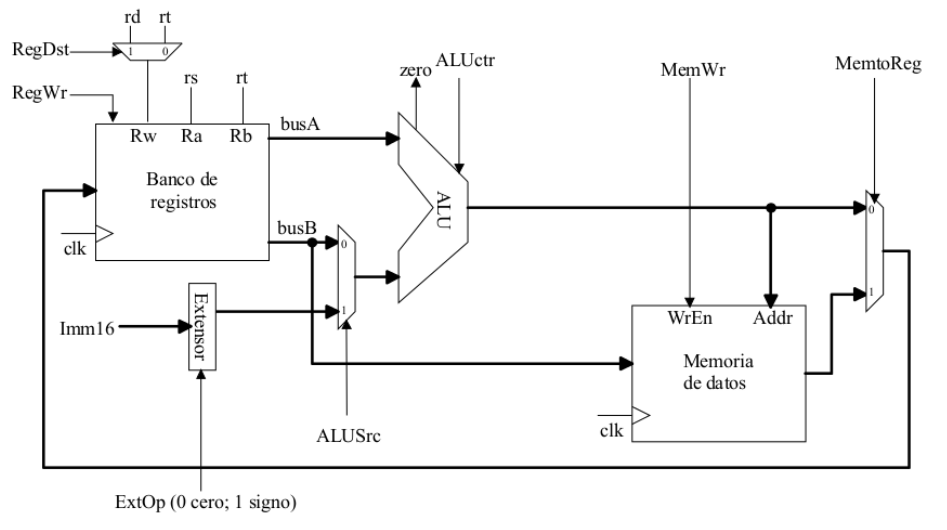
\includegraphics[width=0.88\textwidth,keepaspectratio=true]{unic}
\end{center}
\caption{Procesador Uniciclo}
\end{figure}

\begin{table}[H]
\begin{center}
\begin{tabular}{|c|c|c|c|c|c|c|c|c|} \hline
            & R-type  & ori & andi & lw & sw & beq &  & \\ \hline
RegDst      & 1       & 0   &0     & 0  & x  & x   &  &  \\ \hline
ALUSrc      & 0       & 1   &1     & 1  & 1  & 0   &  &  \\ \hline
MemtoReg    & 0       & 0   &0     & 1  & x  & x   &  &  \\ \hline
RegWr       & 1       & 1   &1     & 1  & 0  & 0   &  &  \\ \hline
MemWr       & 0       & 0   &0     & 0  & 1  & 0   &  &  \\ \hline
nPC\_sel     & 0       & 0   &0     & 0  & 0  & 1   & &  \\ \hline
ExtOp       & x       & 0   &0     & 1  & 1  & x   &  &  \\ \hline
ALUOp       & func    & or  &and   & add& add& sub & & \\ \hline
  &        &    &    &   &   &    &  &  \\ \hline
  &        &    &    &   &   &    &  &  \\ \hline
   &        &    &    &   &   &    &  &  \\ \hline
\end{tabular}
\end{center}
\caption{Señales de control proc. uniciclo}
\end{table}

\newpage

\begin{figure}[H]
\begin{center}
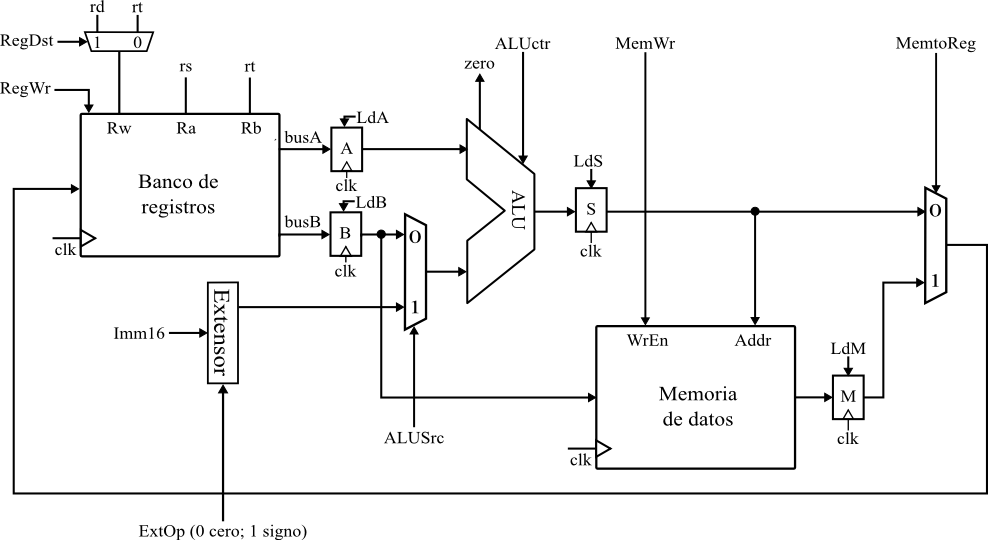
\includegraphics[width=0.88\textwidth,keepaspectratio=true]{proc}
\end{center}
\caption{Procesador Multiciclo}
\end{figure}


\begin{table}[H]
\begin{center}
\begin{tabular}{|c|c|c|c|c|c|c|} \hline
        &(1)&(2)&(3)&(4)&(5) \\ \hline
LdIR    &  &  &  &  &    \\ \hline
RegDst  &  &  &  &  &    \\ \hline
RegWr   &  &  &  &  &    \\ \hline
LdA     &  &  &  &  &    \\ \hline
LdB     &  &  &  &  &    \\ \hline
ExtOp   &  &  &  &  &    \\ \hline
ALUSrc  &  &  &  &  &    \\ \hline
ALUCtr  &  &  &  &  &    \\ \hline
LdS     &  &  &  &  &    \\ \hline
MemWr   &  &  &  &  &    \\ \hline
LdM     &  &  &  &  &    \\ \hline
MemtoReg&  &  &  &  &    \\ \hline
    &  &  &  &  &    \\ \hline
    &  &  &  &  &    \\ \hline

\end{tabular}
\end{center}
\caption{Señales de control por ciclo de instrucción}
\end{table}

\end{document}
